\documentclass[a4paper,10pt,twoside,twocolumn]{dndbook} %a4, 10pt, book (idk why i did that...), 2 cols, dnd-themed
\usepackage[english]{babel} %language
\usepackage[utf8]{inputenc} %lovely utf-8
\usepackage{graphicx} %images
\usepackage{wrapfig} %images
\usepackage{array} %allways use this shit, idk why
\usepackage{tikz} %draw stuff
\usepackage{ifthen} %draw stuff
\usetikzlibrary{shapes,calc,fadings} %draw stuff
\usepackage{xspace} %usefull idk, allways import this stuff
\usepackage{dirtytalk} %\say because fuck it
\usepackage{setspace} %don't ask, kind of like it...
\usepackage{pgfplots}

\usepackage[singlelinecheck=false]{caption} %idk dndbook...
\usepackage{listings} %idk dndbook...
\usepackage{shortvrb} %not used yet...
\usepackage{stfloats} %idk dndbook
\usepackage{dirtytalk}

\singlespacing
\makeatletter %because of titlepage and \HUGE

\@openrightfalse %no empty pages

\graphicspath{ {./images/} }

\def \license {GNU Free Documentation License}
\def \licensetext {Please consider and respect the copyleft of this license. The content of this document should be accessible to everyone. Everyone has the right to use the content of this document as he/she wishes, to modify it, to publish it modified (taking into account the copyleft) and to republish it without any changes (taking into account the copyleft).}
\def \author {Sven Hugi}%if you edit this document, add your name... <3
\def \illustrators {} %add name
\def \othercontrib {} %add name

%highlighting with some random effect -> looks handmade and i love it...
\newcommand\hl[2][yellow]{
	\begin{tikzpicture}[
	baseline,
	decoration={random steps,amplitude=1pt,segment length=15pt},
	outer sep=-15pt, inner sep = 0pt
	]
	\node[decorate,rectangle,fill=#1,anchor=text]{#2\xspace};
	\end{tikzpicture}
}
%2 column layout hack...
\newcommand{\nextPage}{
	\newpage
	\hbox{}
	\newpage
}
%make bad things look ok...
\newcommand{\doublelinebreak}{
	\linebreak\linebreak
}
%the old HUGE fontsize
\newcommand\HUGE{\@setfontsize\Huge{60}{80}} 

\renewcommand{\maketitle}{
	\thispagestyle{empty}
	\onecolumn %fuck it
	\vspace*{5cm}
	\begin{center}
		$\vspace*{2cm}$
			{\HUGE\DndFontDropCap{WOOD WOAD}}\\	
	\end{center}
	\twocolumn %reset shit
}\makeatother

\begin{document}
	\maketitle
	\section*{Credits}
	\vspace{.25cm}
	\textbf{Authors:} \author\linebreak
	\textbf{Illustrators:} \illustrators\linebreak
	\textbf{Additional Contributors:} \othercontrib\linebreak
	\textbf{License:} \license\doublelinebreak
	\licensetext\doublelinebreak
	Image from Cory Trego-Erdner (https://www.artstation.com/corytregoerdner)
	\vfill\pagebreak\hbox{}\vfill\hfill{\tiny This Document was written in \LaTeX.}\pagebreak\vfill\pagebreak

	\vfill\pagebreak
	\section{Wood Woad Traits}
	\textbf{Ability Score Increase.} Your Constitution score increases by 2 and your Wisdom score increases by 1.\linebreak
	\textbf{Age.} Sprouting 3 days after the ritual completes, wood woads mature into their humanoid shape very quickly over a few months, and can exist seemingly indefinitely unless destroyed.\linebreak
	\textbf{Alignment.} They tend towards lawful neutral.\linebreak
	\textbf{Size.} Wood Woad's stand between 4 and 7 feet tall and average about 300 pounds. Your size is Medium.\linebreak
	\textbf{Speed.} Your base walking speed is 30ft.\linebreak
	\textbf{Language.} You can read, write and speak Sylvan and Common.\linebreak
	\textbf{Vulnerability.} Fire\linebreak
	\textbf{Living Plant.} You count as a plant type creature.\linebreak
	\textbf{Plant Camouflage.} You have advantage on Dexterity (Stealth) checks in any terrain with ample obscuring plant life.\linebreak
	\textbf{Darkvision.} You can see in dim light within 60 feet of you as if it were bright light, and in darkness as if it were dim light. You can't discern color in darkness, only shades of gray.\linebreak
	\textbf{Photosynthesis.} Instead of eating or sleeping, you benefit from a long rest after 4 hours staying at one spot, absorbing water, nutrients, air, and bright light to perform photosynthesis.
	\textbf{Defensive.} If you take the dodge action, you benefit from a adittional +5 ac against non magical bludgening, piercing and slashing damage.\linebreak
	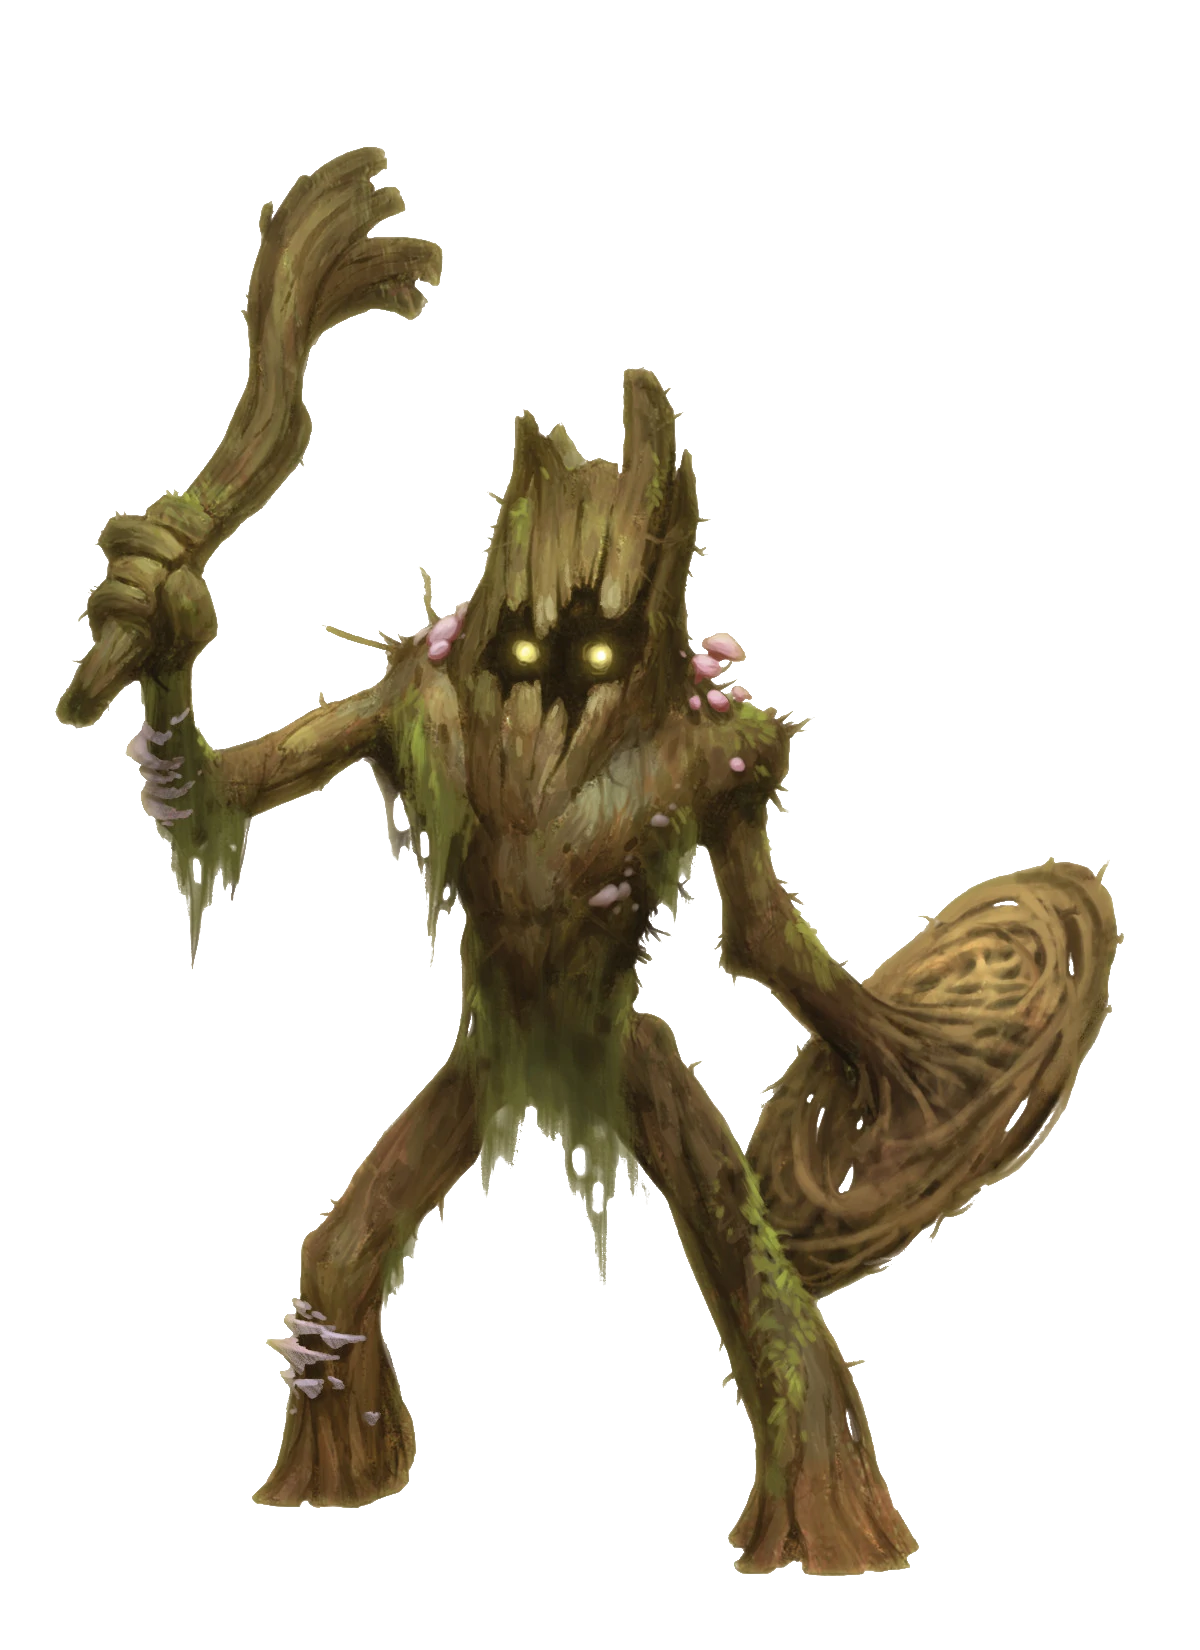
\includegraphics[width=\linewidth]{woodwoad.png}
	
\end{document}